\documentclass[11pt, oneside]{article} 
\usepackage{geometry}
\geometry{letterpaper} 
\usepackage{graphicx}
	
\usepackage{amssymb}
\usepackage{amsmath}
\usepackage{parskip}
\usepackage{color}
\usepackage{hyperref}

\graphicspath{{/Users/telliott/Github/calculus_book/png/}}
% \begin{center} 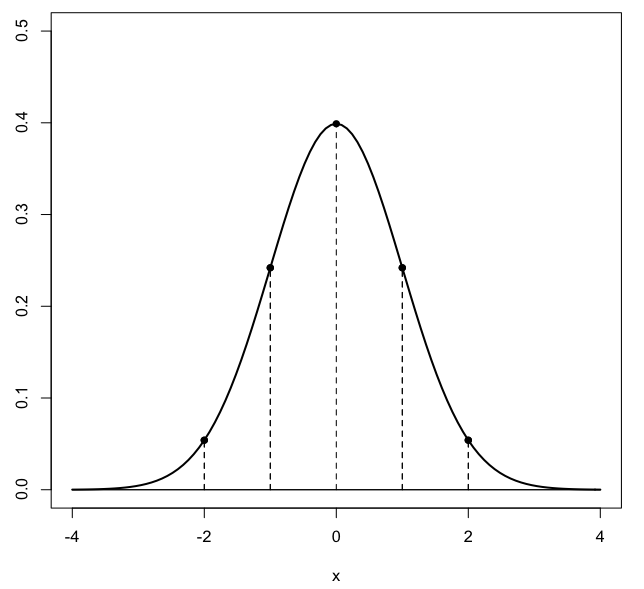
\includegraphics [scale=0.4] {gauss3.png} \end{center}

\title{Natural Numbers}
\date{}

\begin{document}
\maketitle
\Large
\section*{Integers}

The \emph{natural} or counting numbers which everyone learns very early in life are $1, 2, 3$ and so on.

One can get hung up on the question of whether the natural numbers would exist without the problem of counting three sheep or all ten of our fingers.  Leopold Kronecker famously said "God made the integers; all else is man's handiwork".

We will not worry about where they come from.

Mathematicians refer to the \emph{set} of natural numbers and give the set a special symbol, $\mathbb{N}$.  We write
\[ \mathbb{N} = \{ 1, 2, 3 \dots \} \]

The brackets contain between them the elements or members of the set. The dots mean that this sequence continues forever.

How can we decide whether a particular $n$ is in the set if we can't enumerate all of its members?  We can tell by its form whether some $n$ is a natural number or not.  

If this seems problematic, you might call $\mathbb{N}$ a class instead (Hamming);  we carry out \emph{classification} to decide whether $n$ is a natural number.

The notion of an unending sequence can be unnerving upon first encounter.

\subsection*{construction of N}

To construct the set $\mathbb{N}$, start with the smallest element, $1$.  Then 
\[ 1 + 1 = 2, \ \ \ \ \ \ 2 + 1 = 3, \ \ \ \ \ \ 3 + 1 = 4 \dots \]
Add successive elements by forming $a_n + 1 = a_{n+1}$.

$\mathbb{N}$ is an infinite set.

We say there is no largest number in $\mathbb{N}$, no largest $n \in \mathbb{N}$.  The symbol $\in$ means "in the set" or "is a member of the set".

Proof:  suppose $\mathbb{N}$ did have a largest number, $M$.  Well, what about $M + 1$?  By the definition we can construct it, and it is clearly also a member of the set, but $M + 1 > M$ so $M$ is not the largest number in the set.

This is a proof by contradiction that $\mathbb{N}$ is infinite.

$\square$

\subsection*{set membership}

Sometimes people say that
\[ 0 \in \mathbb{N} \]
(0 is a part of the set) but most do not, and we will follow the definition given above.  If you wanted to be explicit about this you could write
\[ 0 \notin \mathbb{N} \]

What do we mean by infinity?  We mean an upper bound on the natural numbers, and later, all real numbers.  

All numbers $n \in \mathbb{N}$ have the property that $n$ is contained in the interval $[1..\infty)$.  However, $\infty$ is \emph{not} part of the interval, and that is the meaning of the the right parenthesis.

$\infty$ is not a number so it probably doesn't even make sense to write $\infty \notin \mathbb{N}$.

\subsection*{least element}

$\mathbb{N}$ does not have a greatest number, but it does have a smallest or least one.  If pairwise comparisons are carried out, a single element, the number $1$, has the property that $1 \le n$ for all numbers $n \in \mathbb{N}$.  As we go on, we will find that other types of numbers (rationals and real numbers), do not have a least positive number.

\subsection*{well-ordered property}

Since we can also find the least member of the set excluding $1$, written $\mathbb{N} \setminus 1$, we can order every number in $\mathbb{N}$.  

This property is called the \textbf{well-ordered} property.

\subsection*{the Integers}

The set $\mathbb{Z}$ contains all the members of $\mathbb{N}$ plus their negatives, as well as the special number $0$, often called the additive identity since $0 + n = n$ for all $n \in \mathbb{N}$.

\[ \mathbb{Z} = \{ \dots -2, -1, 0, 1, 2, \dots \} \]

$\mathbb{Z}$ stands for the German word \emph{Zahlen}, Number.  The set $\mathbb{Z}$ are usually referred to as the integers.

$\mathbb{Z}$ is also an infinite set and also has the well-ordered property.  To show this simply order all numbers $p > 0$ with respect to zero using $<$, and all the numbers $n < 0$ using $>$.

\subsection*{inequality}
You have surely seen and used the symbols $>$ (greater than), and $<$ (less than).

Among the axioms of the number systems is the collection of \emph{order axioms}.  A few definitions:

$\circ$ \ $x < y$ means that $y - x$ is positive

$\circ$ \ $y > x$ means that $x < y$

For arbitrary numbers $a$ and $b$ only one of three statements is true:  

$a < b$, $a = b$ or $a > b$.

There is no need to be systematic here.  Let us just mention that these properties (and their kin) are true not just for natural numbers, but also for the rational numbers and the real numbers, which we will get to soon.  

Here are a few important theorems about order which we will use:

$\circ$ \ If $a < b$, and $c$ is any number, then $a + c < b + c$

$\circ$ \ If $a < b$, then $-b < -a$

$\circ$ \ If $a < b$ and $c > 0$, then $ac < bc$

The first one above implies the second and the third.

\subsection*{algebraic operations}

$\circ$ addition:  $a + b$

$\circ$ subtraction:  $a - b = a + (-b)$

The negative integers and $0$ solve the problem of how to evaluate $a - b$ when $b \ge a$.

$\circ$ multiplication:  $a \cdot b$, also often written $ab$ (but not $a \times b$, at this level).

And then:

$\circ$ division $a/b$, equivalent to finding a number $c$ such that $c \cdot b = a$.

\subsection*{algebra}
As you know, the basic axioms of algebra include the following:

$\circ$ \ Commutativity for addition and multiplication: 
\[ a + b = b + a, \ \ \ \ \ \ a \cdot b = b \cdot a \]

$\circ$ \  Associativity for addition and multiplication:
\[ (a + b) + c = a + (b + c), \ \ \ \ \ \ (a \cdot b) \cdot c = a \cdot (b \cdot c) \]

$\circ$ \ Distributivity of addition over multiplication:  
\[ a \cdot (b + c) = a \cdot b + a \cdot c \]

$\circ$ \ Additive identity:  $0 + a = a$.

$\circ$ \ Multiplicative identity:  $1 \cdot a = a$.


\end{document}